
\documentclass[12pt,letterpaper,twoside]{article}


% Packages
\usepackage[spanish]{babel}
\usepackage{caption}
\usepackage[sfdefault,lf]{carlito}
\usepackage{datetime}
\usepackage{fancyhdr}
\usepackage{float}
\usepackage[T1]{fontenc}
\usepackage{geometry}
\usepackage{graphicx}
\usepackage[hidelinks]{hyperref}
\usepackage[utf8]{inputenc}
\usepackage{listings}
\usepackage{longtable}
\usepackage{multirow}
\usepackage{newfloat}
\usepackage{totcount}
\usepackage[table]{xcolor}
\usepackage{xurl}

% Macros
\newcommand{\printif}[3]{\ifcsname @#1\endcsname#2\else#3\fi}

% Variables
\makeatletter
  \def\institution#1{\gdef\@institution{#1}}
  \def\classcode#1{\gdef\@classcode{#1}}
  \def\classname#1{\gdef\@classname{#1}}
  \def\classsemester#1{\gdef\@classsemester{#1}}
  \def\classparallel#1{\gdef\@classparallel{#1}}
  \def\doctitle#1{\gdef\@doctitle{#1}}
  \def\docsubtitle#1{\gdef\@docsubtitle{#1}}
  \def\version#1{\gdef\@version{#1}}
  \def\astudentname#1{\gdef\@astudentname{#1}}
  \def\astudentlastname#1{\gdef\@astudentlastname{#1}}
  \def\astudentrol#1{\gdef\@astudentrol{#1}}
  \def\astudentemail#1{\gdef\@astudentemail{#1}}
  \def\bstudentname#1{\gdef\@bstudentname{#1}}
  \def\bstudentlastname#1{\gdef\@bstudentlastname{#1}}
  \def\bstudentrol#1{\gdef\@bstudentrol{#1}}
  \def\bstudentemail#1{\gdef\@bstudentemail{#1}}
  \def\cstudentname#1{\gdef\@cstudentname{#1}}
  \def\cstudentlastname#1{\gdef\@cstudentlastname{#1}}
  \def\cstudentrol#1{\gdef\@cstudentrol{#1}}
  \def\cstudentemail#1{\gdef\@cstudentemail{#1}}
\makeatother

% Page geometry
\geometry{
  letterpaper,
  top=1.0in,
  bottom=1.0in,
  left=1.25in,
  right=1.25in,
  headheight=15pt,
}
\setlength\parskip{1em}
\setlength\parindent{15pt}
\DeclareCaptionFormat{elements}{\captionsetup{justification=justified}\textbf{#1#2}#3\par}

% Header and footer
\pagestyle{fancy}
\cfoot{\thepage}
\renewcommand{\headrulewidth}{0.5pt}
\renewcommand{\footrulewidth}{0.5pt}
\makeatletter
  \fancyhead[LE]{\printif{classcode}{\@classcode\ - }{}\@classsemester}
  \fancyhead[RE]{\@doctitle}
  \fancyhead[LO]{\@astudentlastname\printif{bstudentlastname}{, \@bstudentlastname}{}\printif{cstudentlastname}{, \@cstudentlastname}{}}
  \fancyhead[RO]{\printif{version}{\@version\ - }{}\the\year/\two@digits{\month}/\two@digits{\day}}
\makeatother

% Tables configuration
\regtotcounter{table}

\captionsetup[table]{name=Tabla}
\captionsetup[table]{format=elements, singlelinecheck=false, margin=0pt, font={sf,footnotesize}}

% Figures configuration
\regtotcounter{figure}
\graphicspath{{figures/}}
\captionsetup[figure]{format=elements, singlelinecheck=false, margin=0pt, font={sf,footnotesize}}

% Code configurations
\DeclareFloatingEnvironment[fileext=loc]{code}
\regtotcounter{lstlisting}
\renewcommand\lstlistingname{Código}
\captionsetup[lstlisting]{format=elements, singlelinecheck=false, margin=0pt, font={sf,footnotesize}}
\lstset{
    inputencoding=utf8,
    extendedchars=true,
    literate=%
    {á}{{\'a}}1
    {é}{{\'e}}1
    {í}{{\'i}}1
    {ó}{{\'o}}1
    {ú}{{\'u}}1
    {Á}{{\'A}}1
    {É}{{\'E}}1
    {Í}{{\'I}}1
    {Ó}{{\'O}}1
    {Ú}{{\'U}}1
    {ñ}{{\~n}}1
    {Ñ}{{\~N}}1
}
\lstset{
    basicstyle=\small\ttfamily,
    backgroundcolor=\color{gray!10},
    keywordstyle=\color{blue},
    commentstyle=\color{green!40!black},
    stringstyle=\color{red},
    rulecolor=\color{gray},
    frame=single,
    framerule=0pt,
    framesep=2pt,
    captionpos=b,
    aboveskip=10pt,
    belowskip=5pt,
    columns=fullflexible,
    keepspaces=true,
    numberstyle=\tiny\color{gray},
    numbers=left,
    stepnumber=1,
    numbersep=5pt,
}
\lstdefinestyle{pythonstyle}{
    language=python
}
\lstnewenvironment{pythoncode}{\lstset{style=pythonstyle}}{}
\lstdefinestyle{bashstyle}{
    language=bash
}
\lstnewenvironment{bashcode}{\lstset{style=bashstyle}}{}
\lstdefinestyle{xmlstyle}{
    language=xml
}
\lstnewenvironment{xmlcode}{\lstset{style=xmlstyle}}{}
\lstdefinestyle{javastyle}{
    language=java
}
\lstnewenvironment{javacode}{\lstset{style=javastyle}}{}
\lstdefinestyle{plainstyle}{
}
\lstnewenvironment{plaincode}{\lstset{style=plainstyle}}{}

% Custom titlepage
\makeatletter
\def\@maketitle{
  % Configurations
  \renewcommand\listtablename{Índice de tablas}
  \renewcommand\lstlistlistingname{Índice de fragmentos de codigo}
  % Cover
  \thispagestyle{empty}
  \noindent\includegraphics[width=.475 \textwidth]{../latex-report-001/logo-\@institution}
  \vfill
  \vfill
  \begin{center}
    \printif{docsubtitle}{\fontsize{25}{25}\selectfont \@docsubtitle\\[3em]}{}
    {\fontsize{35}{35}\selectfont \@doctitle}\\[2.0em]
    {\fontsize{15}{15}\selectfont \printif{classcode}{\@classcode\ - }{}\@classsemester\printif{classparallel}{ - \@classparallel}{}}\\[10pt]
    {\fontsize{20}{20}\selectfont \@classname}\\[5pt]
    {\fontsize{15}{15}\selectfont \today\printif{version}{ - \@version}{}}
  \end{center}
  \vfill
  \vfill
  \vfill
  \begin{flushright}
    \begin{tabular}{r|l}
      \printif{astudentname}{\@astudentname\ \@astudentlastname & \@astudentrol \\ \@astudentemail & \\}{}
      \printif{bstudentname}{\@bstudentname\ \@bstudentlastname & \@bstudentrol \\ \@bstudentemail & \\}{}
      \printif{cstudentname}{\@cstudentname\ \@cstudentlastname & \@cstudentrol \\ \@cstudentemail & \\}{}
    \end{tabular}
  \end{flushright}
  \newpage
  % Index
  % Table of contents
  \tableofcontents
  % Tables
  \ifnum \totvalue{table}>0
    \listoftables
  \fi
  % Figures
  \ifnum \totvalue{figure}>0
    \listoffigures
  \fi
  % Code
  \ifnum \totvalue{lstlisting}>0
    \lstlistoflistings
  \fi
  \newpage
}
\makeatother

% Hooks
\AtBeginDocument{
  \maketitle
}


% Datos de la asignatura
\institution{utfsm}
\classcode{INF356}
\classname{Computación Distribuida para Big Data}
\classsemester{2025-1}
\classparallel{200}

% Datos de la entrega
\doctitle{Trabajo Práctico 2}
\version{v1.0}

% Estudiante
\astudentname{Miguel}
\astudentlastname{Soto}
\astudentrol{201973623-K}
\astudentemail{miguel.sotod@sansano.usm.cl}
  
\begin{document}

%%%%%%%%%%%%%%%%%%%%%%%%%%%%%%%%%%%%%%%%%%%%%%%%%%%%%%%%%%%%%%%%%%%%%%%%%%%%%%%%%%%
% Borrar o comentar esta sección instrucciones antes de entregar %%%%%%%%%%%%%%%%%%
%%%%%%%%%%%%%%%%%%%%%%%%%%%%%%%%%%%%%%%%%%%%%%%%%%%%%%%%%%%%%%%%%%%%%%%%%%%%%%%%%%%

\section{Map Reduce}

\noindent
Esta entrega consistia en modificar el codigo fuente de Hadoop para agregar funcionalidad extra, en donde habia que implementar metodos a partir de la funcion WordCount.

\noindent
Se pedia que crear una funcion que permitiese contar palabras previamente filtradas a partir de reglas indicadas en el informe.

\noindent
Luego, habia que crear otra funcion que permitiese extraer columnas de la salida de WordCount a partir del indice de la columna.

\noindent
Por motivos de eficiencia y por simplicidad, opte por parchar el codigo binario de Hadoop con las clases nuevas creadas a partir de WordCount en las funciones
de ejemplo originales, de esta forma pude invocarlas facilmente y no tener que compilar el codigo fuente cada vez que hiciera un cambio en el codigo.

\noindent
Grabe un video explicativo mostrando el proceso en ejecucion junto a las salidas de ambos programas, ya que en el practico inicial fue recurrente el tema de que no
dejar evidencia clara de los puntos que iba desarrollando. Aqui deje el {\color{blue}\href{https://www.youtube.com/watch?v=UVJUVDU4luk}{enlace}} al video en YouTube.

\newpage

\subsection{Implementación extendida de wordcounter}

\noindent
Para desarrollar esta nueva funcionalidad me base en la implementacion de la clase original de WordCount, la cual obtuve desde el repositorio publico de Apache Hadoop
en GitHub ({\color{blue}\href{https://github.com/apache/hadoop}{enlace}}), en donde dicha funcion se encuentra en la carpeta de ejemplos.

\noindent
La forma en la que luego parche el codigo, fue aprovechandome de los .jar que contiene el binario de Hadoop, estos ultimos son esencialmente
archivos comprimidos que contienen los archivos .class de todas las clases .java de la fuente. Mas aun, el comando jar tiene la funcionalidad
de actualizar un .jar con clases nuevas o con modificaciones de estas. Esto se puede lograr de la siguiente manera:

\begin{figure}
    \centering
    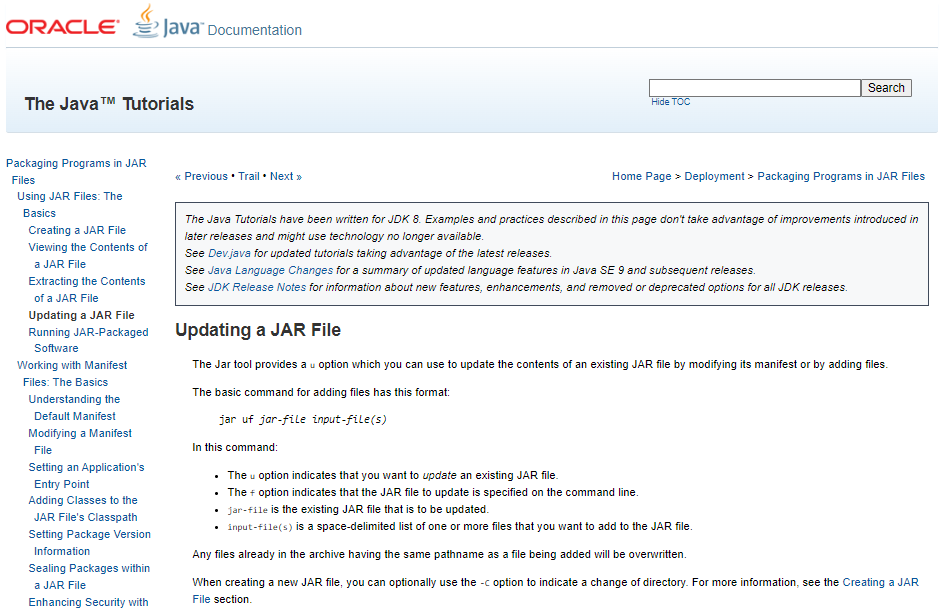
\includegraphics[width=\textwidth]{oracle-jar.PNG}
    \caption{Documentacion oficial de Oracle sobre como parchar un JAR}
    \label{hdfs.PNG}
\end{figure}

\noindent
A continuacion dejare el codigo original de WordCount y el codigo de ExtendedWordCount, hecho a partir del anterior.

\newpage

\begin{code}[H]
    \lstinputlisting[style=javastyle, caption={Codigo original de WordCount}, label={lst:002}]{code/WordCount.java}
\end{code}

\newpage

\begin{code}[H]
    \lstinputlisting[style=javastyle, caption={Codigo de ExtendedWordCount}, label={lst:002}]{code/ExtendedWordCount.java}
\end{code}

\newpage

\subsection{Implementación de selector de columna}

De la misma manera que el punto anterior, me base en WordCount para crear el codigo para la clase SelectColumnExtractor, el cual permite sustraer
una columna de la salida de WordCount en base al indice/numero de columna. Esta funcion en particular ejecuta WordCount si lo filtra al terminar
el proceso de Map-Reduce.

\newpage

\begin{code}[H]
    \lstinputlisting[style=javastyle, caption={Codigo de SelectColumnExtractor}, label={lst:002}]{code/SelectColumnExtractor.java}
\end{code}

\newpage

\subsection{Tiempo de ejecución}

\noindent
A continuación se muestran las medidas obtenidas utilizando el comando time en ExtendedWordCount:

\begin{table}[h!]
\centering
\begin{tabular}{lccc}
\toprule
\textbf{Archivo} & \textbf{real (s)} & \textbf{user (s)} & \textbf{sys (s)} \\
\midrule
sw-script-e04.txt  & 0m32.822s  & 0m7.653s & 0m0.388s
\bottomrule
\end{tabular}
\caption{Tiempos de ejecución del WordCount extendido}
\end{table}

\noindent
Luego se muestran las medidas obtenidas utilizando el comando time en SelectColumnExtractor:

\begin{table}[h!]
\centering
\begin{tabular}{lccc}
\toprule
\textbf{Archivo} & \textbf{real (s)} & \textbf{user (s)} & \textbf{sys (s)} \\
\midrule
sw-script-e04.txt  & 0m17.656s  & 0m7.137s & 0m0.350s
\bottomrule
\end{tabular}
\caption{Tiempos de ejecución del SelectColumnExtractor}
\end{table}

\noindent
Comparando ambos resultados, puedo concluir que:
\begin{itemize}
    \item El algoritmo de ExtendedWordCount es más intensivo en CPU, debido al preprocesamiento de texto, pero se mantiene eficiente gracias a la simplicidad del flujo MapReduce.
    \item El SelectColumnExtractor es más ligero y orientado a E/S, siendo más rápido en archivos simples, pero ligeramente mas costoso si las líneas contienen muchas columnas.
    \item Ambas soluciones escalan correctamente, pero el SelectColumnExtractor presenta tiempos de respuesta mas bajos en tareas estructuradas y simples.
\end{itemize}

\noindent
Los resultados se pueden ver en tiempo real en el video indicado al inicio del practico ({\color{blue}\href{https://github.com/apache/hadoop}{enlace}}).

\newpage

\section{Spark}

A continuacion se describe detalladamente el desarrollo de la tarea práctica avanzada de Big Data, basada en el uso de \texttt{Flintrock} para la configuración de un clúster Spark en AWS. 
A diferencia del informe original, este documento se enfoca en detallar todo el proceso personal, incluyendo errores cometidos, correcciones, decisiones de diseño, observaciones y comentarios 
adicionales que pueden ser útiles para otros estudiantes que enfrenten una tarea similar. Se proporciona ademas un video explicativo mostrando evidencia de el levantamiento de el informe y otros
detalles adicionales ({\color{blue}\href{https://www.youtube.com/watch?v=cp5aBbUCwiQ}{enlace}}).

Para comenzar, se utilizó el mismo clúster que se trabajó en la entrega inicial. Se eliminó manualmente todos los nodos worker, manteniendo solamente el nodo master. Este paso fue esencial para asegurar una base limpia antes de implementar una nueva configuración.

Se clonaron los siguientes repositorios proporcionados por el profesor:
\begin{itemize}
    \item \texttt{https://github.com/ptoledo-teaching/training-bigdata-002}
    \item \texttt{https://github.com/nchammas/flintrock}
\end{itemize}

Estos repositorios contienen scripts clave para la creación del clúster. Se realizó una navegación rápida con \texttt{tree} y \texttt{vim} para entender su estructura y funcionalidades.

El proceso de instalación incluyó los siguientes pasos:
\begin{enumerate}
    \item Instalación de \texttt{AWS CLI}.
    \item Instalación de \texttt{pipx}.
    \item Instalación de \texttt{Flintrock} mediante \texttt{pipx}.
\end{enumerate}

Durante este proceso, se descubrió que el script contenía una instrucción para crear un rol IAM para S3, pero el profesor indicó que esto no era necesario. Por ende, se omitió este paso aunque inicialmente se intentó (sin éxito, debido a permisos insuficientes).


Se detectó un bug en la versión actual de Flintrock relacionado con incompatibilidades de Spark. Para solucionarlo, se aplicó un parche manualmente en el código fuente de Flintrock instalado. El procedimiento incluyó:
\begin{itemize}
    \item Edición directa de los archivos indicados por el profesor.
    \item Verificación y corrección de problemas de indentación (uso de tabs vs. espacios).
    \item Uso de expresiones regulares para reemplazo masivo.
\end{itemize}

\textbf{Nota:} Se olvidó hacer un respaldo del archivo original antes de modificar, lo que pudo haber provocado una reinstalación completa en caso de error.

Se creó una nueva clave PEM con permisos adecuados y se renombró según el formato requerido por Flintrock. Inicialmente se cometió un error en los permisos, generando un \texttt{warning}. Posteriormente se corrigió con:

\begin{lstlisting}[language=bash]
chmod 400 clave.pem
\end{lstlisting}

Esto permitió una conexión exitosa al nodo master.

\subsection{Escalamiento vertical y horizontal}

Se procedió a levantar múltiples configuraciones de clúster usando archivos \texttt{.yaml} modificados. Se observó que configuraciones con más de 8 nodos fallaban debido a restricciones de la cuenta de estudiante. Por lo tanto, se trabajó principalmente con configuraciones de hasta 6 nodos \texttt{t3.large}.

\begin{itemize}
    \item Configuración con 10 \texttt{t3.medium} no logró levantar el clúster.
    \item Ejecute el script \texttt{test-000.sh} en lugar de \texttt{test-001.sh}, generando inconsistencias en los benchmarks.
\end{itemize}

\subsection*{Tiempos Registrados}

\begin{longtable}{|c|c|c|}
\hline
\textbf{Configuración} & \textbf{Test Ejecutado} & \textbf{Tiempo Aproximado} \\
\hline
4 \texttt{t3.large} & test-000.sh & 24 (real) \\
\hline
4 \texttt{t3.large} & test-000.sh & 24 (real) \\
\hline
4 \texttt{t3.small} & test-000.sh & 25 (real) \\
\hline
6 \texttt{t3.micro} & test-000.sh & 25 (real) \\
\hline
6 \texttt{t3.small} & test-000.sh & 26 (real) \\
\hline
10 \texttt{t3.medium} & test-000.sh & Falló (fallaba en launch.sh) \\
\hline
\end{longtable}

\textit{Nota:} Los tiempos fueron medidos usando el comando \texttt{time bash test00.sh}, y registrados manualmente en un bloc de notas para su análisis posterior.

\section{Procesamiento de datos}

Al igual que en las entregas anteriores del practico avanzado, el desarrollo fue desarrollado en vivo y se adjunta un video de la demostracion de este a traves de un enlace al video en YouTube ({\color{blue}\href{https://www.youtube.com/watch?v=GdrpnyFULTI}{enlace}}).

En las revisiones de las entregas anteriores se indico que no puse evidencia suficiente, lo cual me sorprendio ya que me di el tiempo de hacer los videos explicitamente porque en la entrega incial fue recurrente el tema de la poca documentacion.

Me gusta creer que quien corrigio mis tareas no vio el link que adjunte y por ende voy a dejar en cada seccion el enlace a la parte especifica del video en donde se muestra el funcionamiento de mi codigo.

\subsection{Extracción, transformación y carga}

Durante el desarrollo del proceso ETL, se utilizó un clúster Spark configurado con seis máquinas tipo \texttt{t3.large} en AWS. Se gestionó todo el código mediante un repositorio GitHub, el cual fue clonado en el nodo \texttt{master} del clúster para facilitar la edición y sincronización.

El procedimiento se organizó en scripts numerados (por ejemplo, \texttt{code-005.py}), con scripts de ejecución asociados (por ejemplo, \texttt{test-005.sh}). Para comenzar, se eliminaron los datos anteriores del bucket S3 estudiantil para asegurar un entorno limpio.

El código leyó las 20 porciones del dataset desde el bucket público, aplicando el esquema correspondiente, uniendo todos los fragmentos en un único \texttt{DataFrame}. Se eliminaron filas con valores nulos y se tomó una muestra del 1\% de los datos para pruebas. Luego, se filtraron las observaciones con \texttt{category = SCIENCE} y \texttt{obs\_type = OBJECT}.

El campo \texttt{template\_start} fue procesado para eliminar la letra \texttt{T} y poder convertirlo a formato Unix. Las coordenadas ecuatoriales se dividieron en grados, minutos y segundos, y se almacenó la información en formato \texttt{Parquet} en el bucket del estudiante bajo el nombre \texttt{vlt\_observations\_etl.parquet}.

\newpage

Evidencia del desarrollo a modo de images y enlace a la seccion del video con la demostracion ({\color{blue}\href{https://youtu.be/GdrpnyFULTI?si=b5H6Qznky7ijbZmJ&t=177}{enlace}}).

\begin{figure}[H]
    \centering
    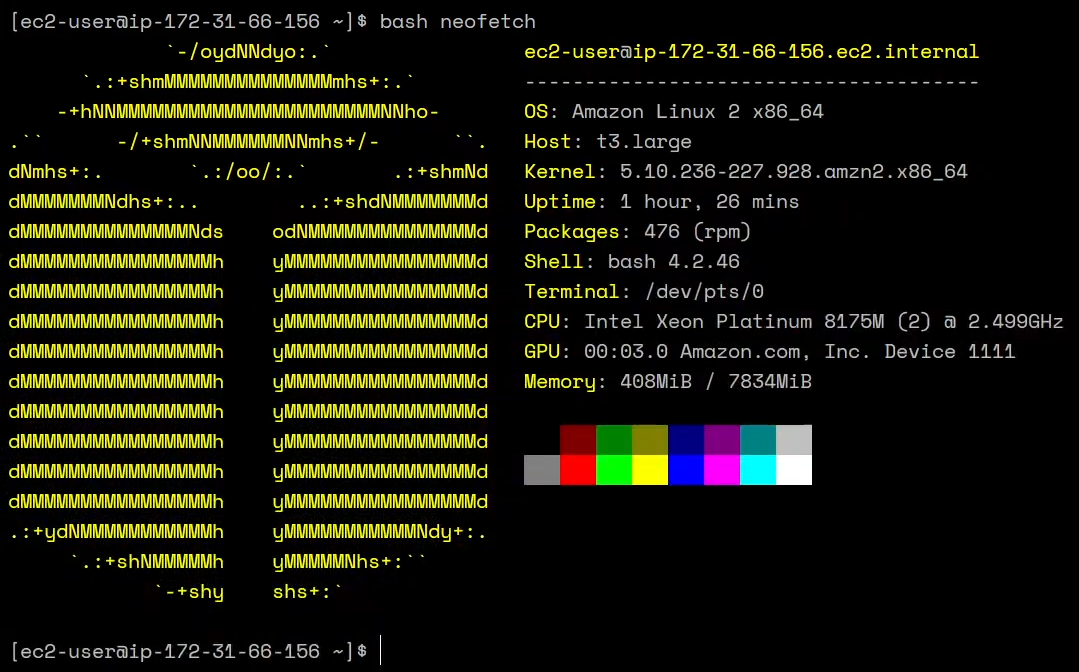
\includegraphics[height=5cm]{31-figura-0.PNG}
    \caption{Neofetch en el nodo master del cluster de Spark}
\end{figure}

\begin{figure}[H]
    \centering
    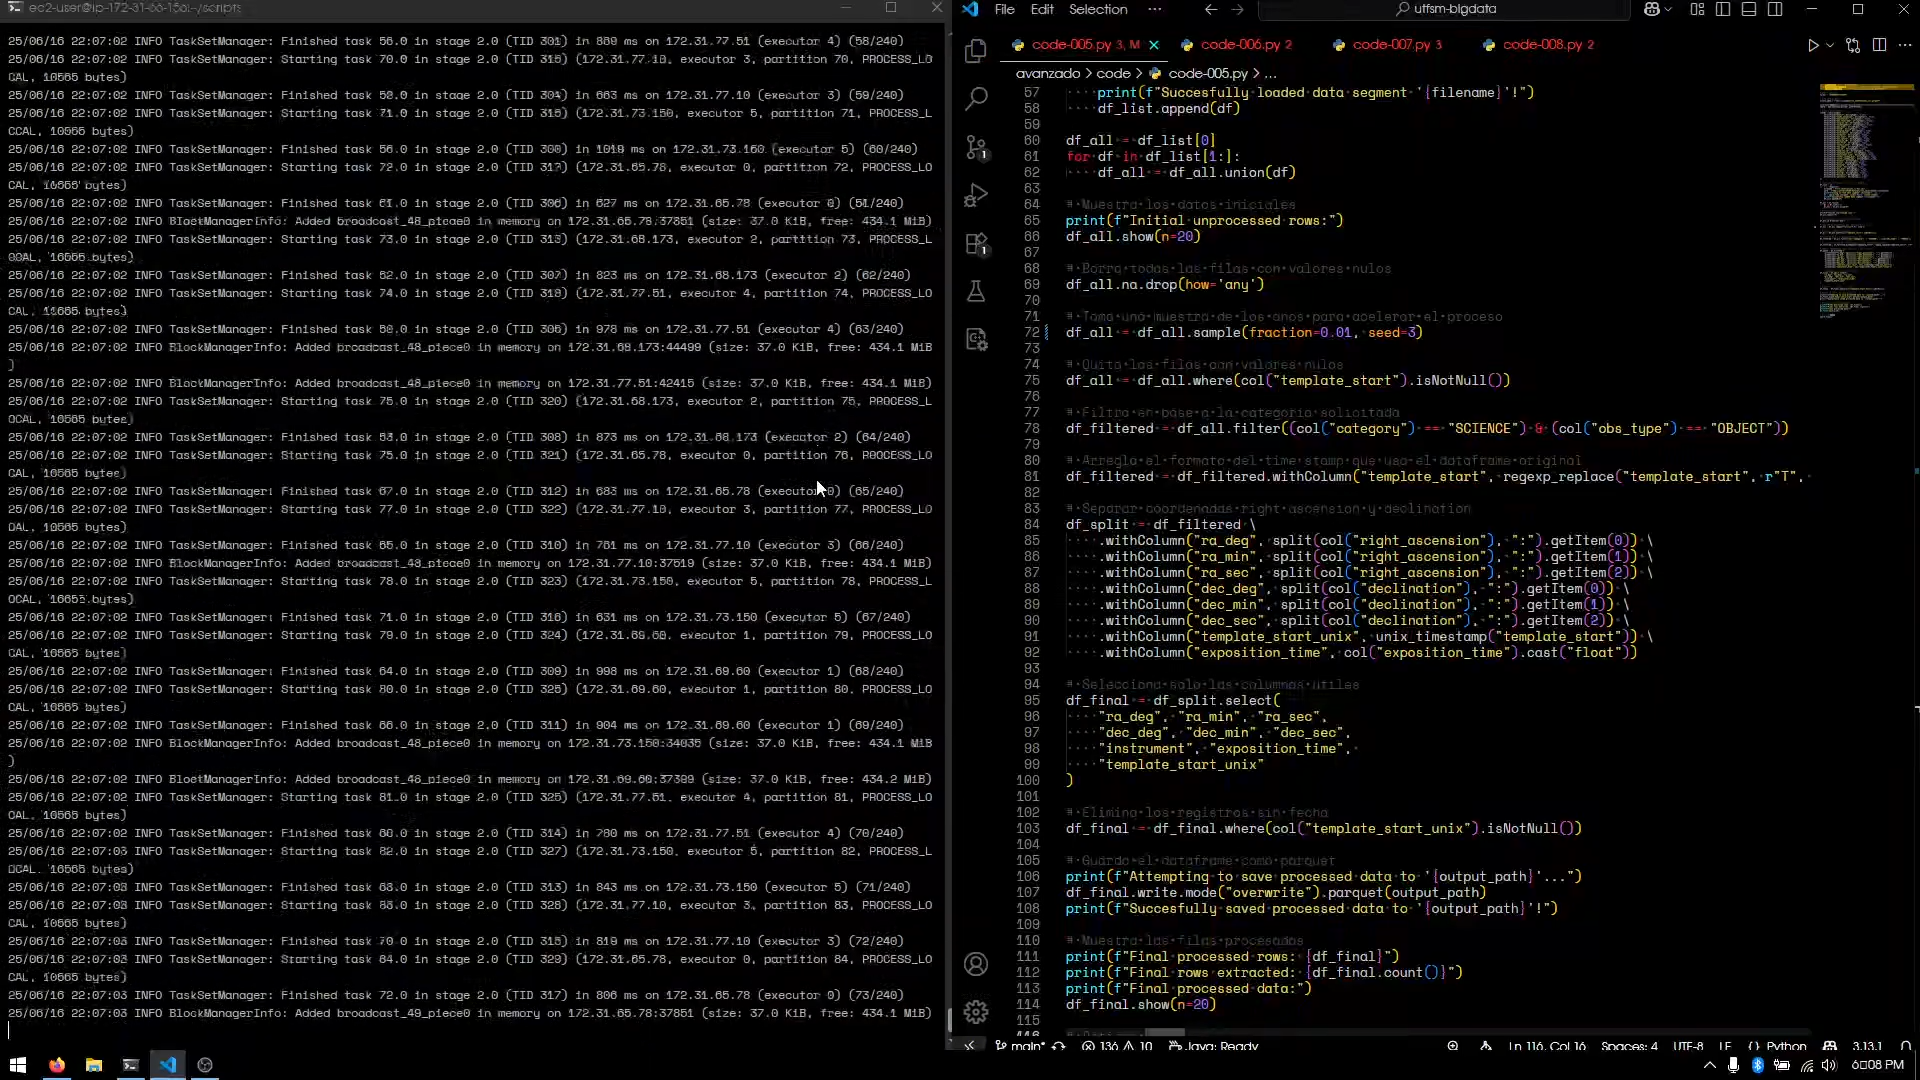
\includegraphics[height=5cm]{31-figura-1.PNG}
    \caption{Spark procesando los datos de esta seccion con el codigo al lado}
\end{figure}

\begin{figure}[H]
    \centering
    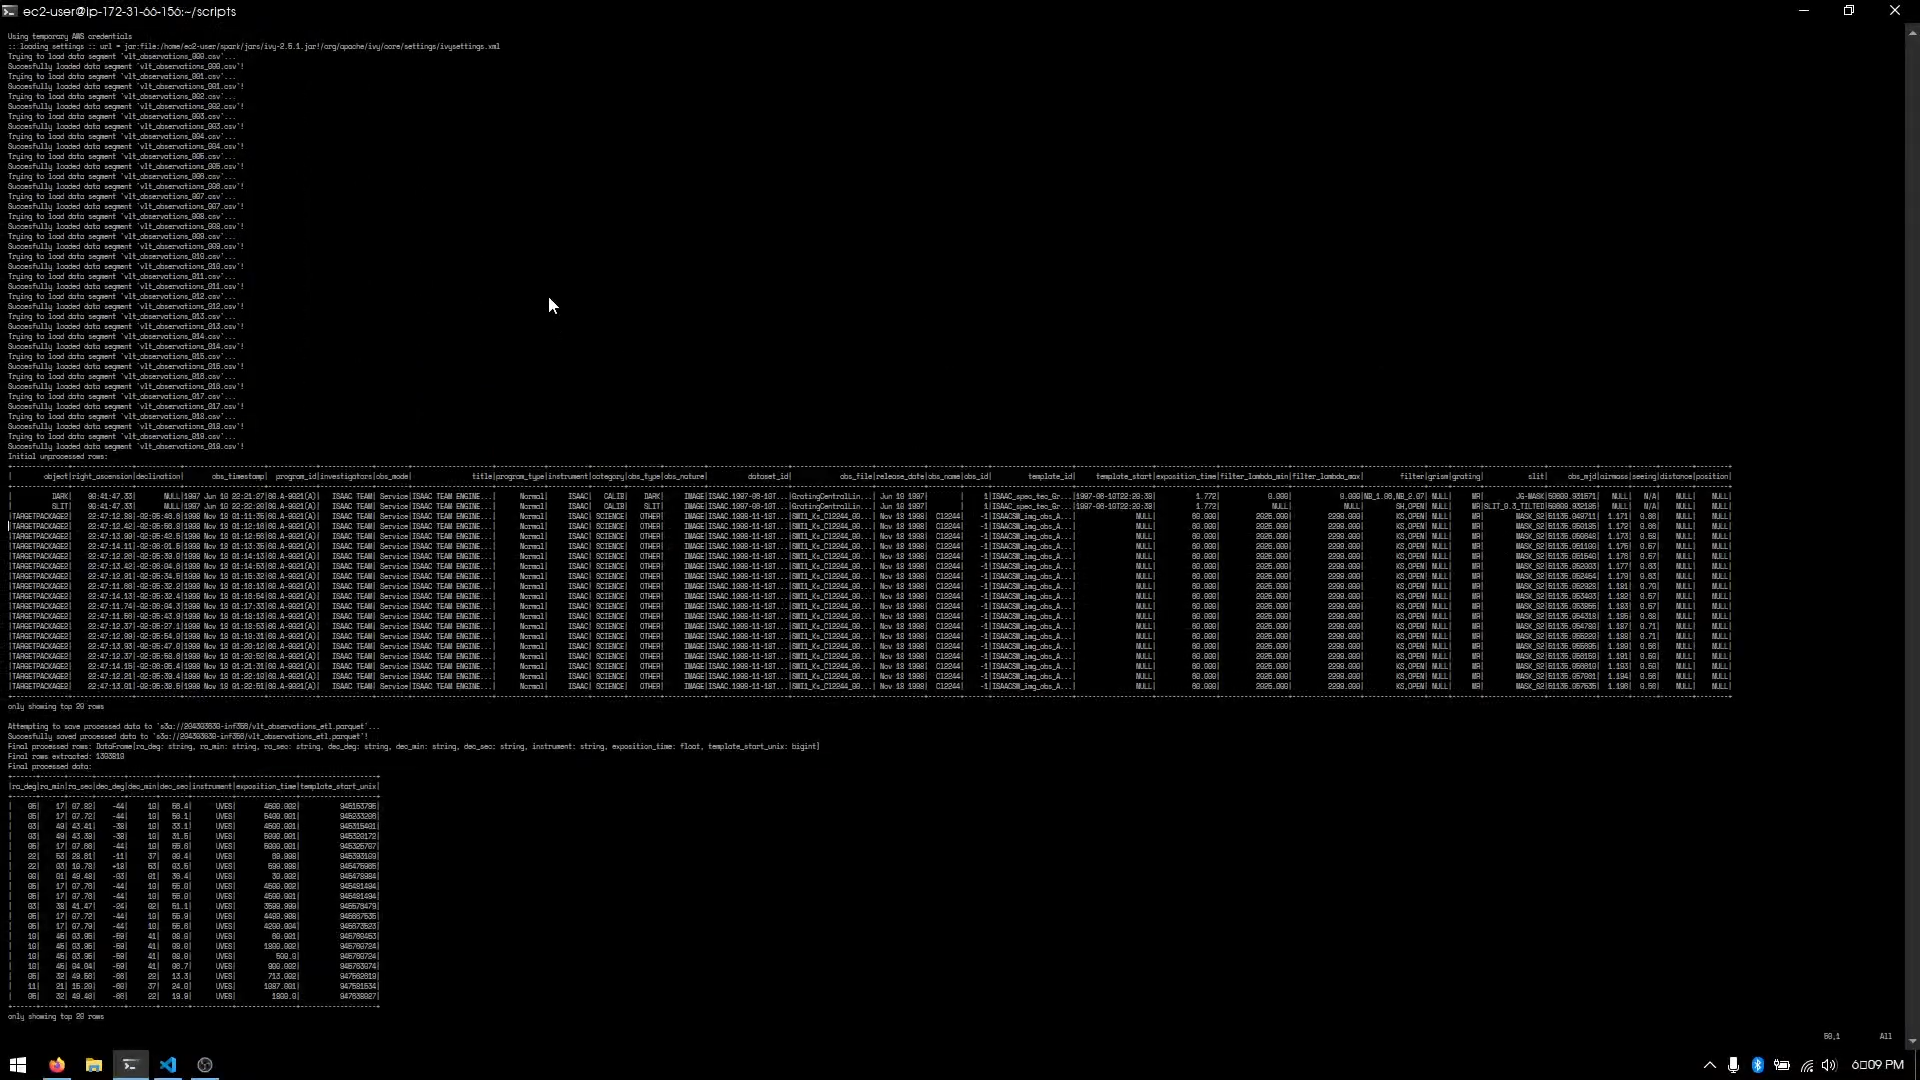
\includegraphics[height=5cm]{31-figura-2.PNG}
    \caption{Dataframe incial y resultante tras procesar los datos}
\end{figure}

\newpage

\begin{figure}[H]
    \centering
    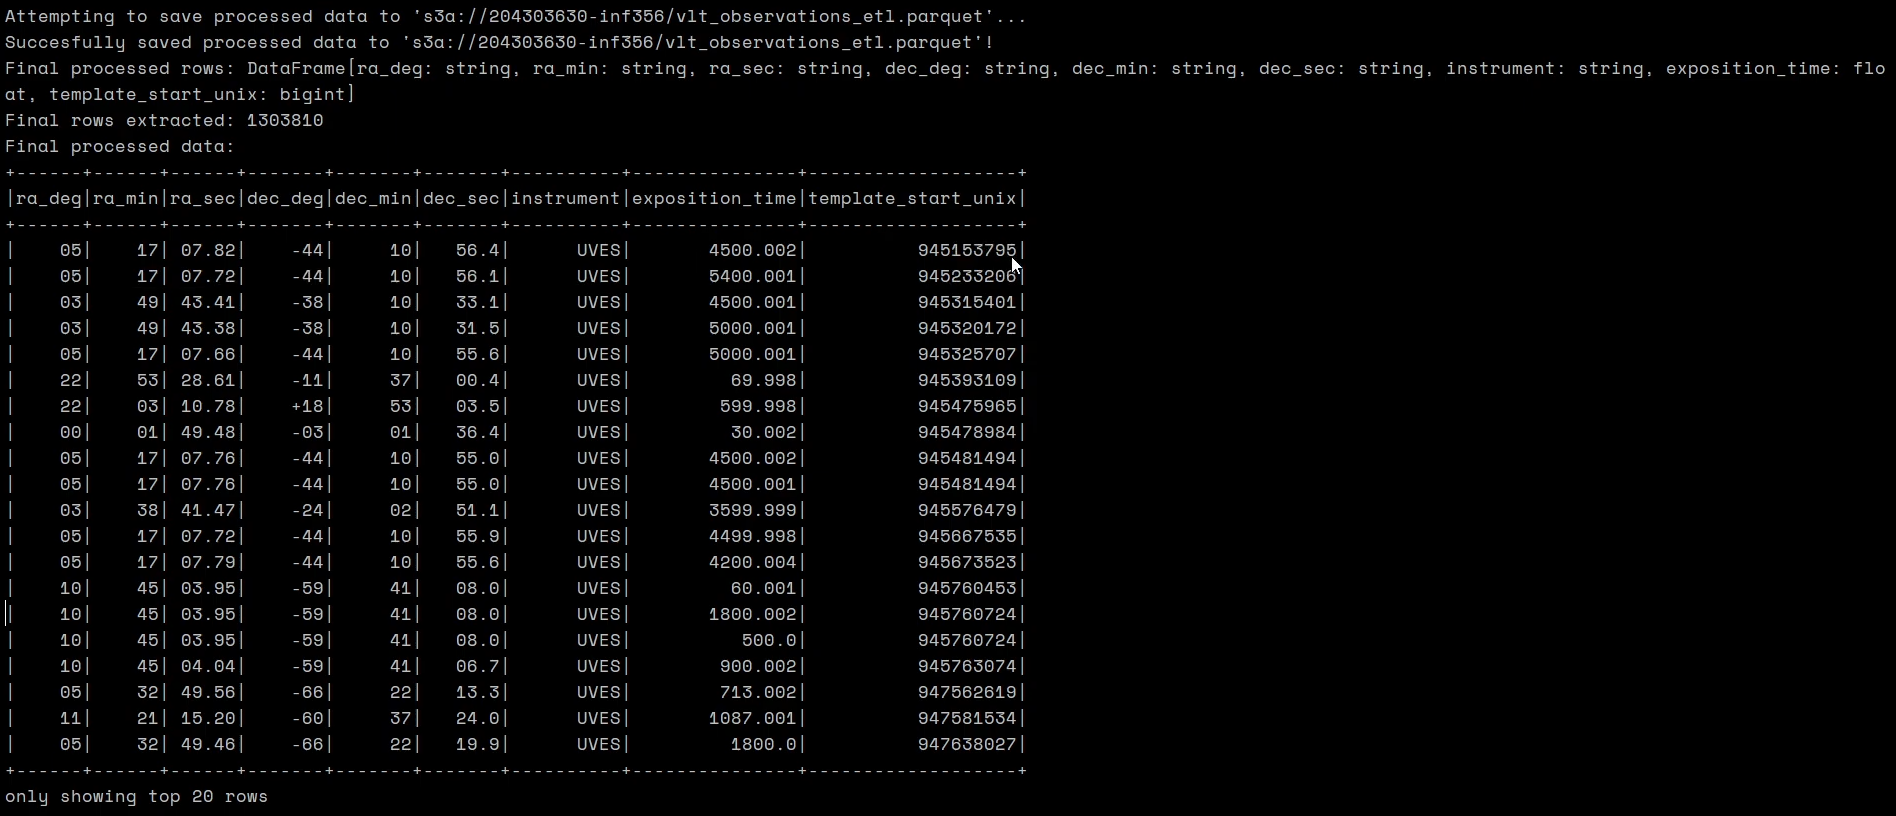
\includegraphics[height=5cm]{31-figura-final.PNG}
    \caption{Dataframe resultante tras procesar los datos}
\end{figure}

\newpage

\begin{code}[H]
    \lstinputlisting[style=pythonstyle, caption={Código utilizado para el procedimiento de ETL}, label={lst:005}]{code/code-005-cut-1.py}
\end{code}

\newpage

\begin{code}[H]
    \lstinputlisting[style=pythonstyle, caption={Código utilizado para el procedimiento de ETL}, label={lst:005}]{code/code-005-cut-2.py}
\end{code}
\newpage
\begin{code}[H]
    \lstinputlisting[style=pythonstyle, caption={Código utilizado para el procedimiento de ETL}, label={lst:005}]{code/code-005-cut-3.py}
\end{code}

\newpage

\subsection{Coordenadas galácticas}

Se desarrolló un programa que transforma las coordenadas ecuatoriales en galácticas a partir del archivo generado en el proceso ETL. Se cargó el archivo \texttt{vlt\_observations\_etl.parquet}, tomando una muestra del 25\% para agilizar el desarrollo.

Se convirtieron las coordenadas de grados, minutos y segundos a grados decimales utilizando cálculos trigonométricos básicos. Luego, se realizaron las transformaciones necesarias para obtener la ascensión recta y declinación galáctica, las cuales fueron almacenadas junto con los campos \texttt{instrument}, \texttt{exposition\_time} y \texttt{template\_start}.

El resultado se guardó en el archivo \texttt{vlt\_observations\_gc.parquet}.

Evidencia del desarrollo a modo de images y enlace a la seccion del video con la demostracion ({\color{blue}\href{https://youtu.be/GdrpnyFULTI?si=cb-NDtVoNadNSFb7&t=466}{enlace}}).

\begin{figure}[H]
    \centering
    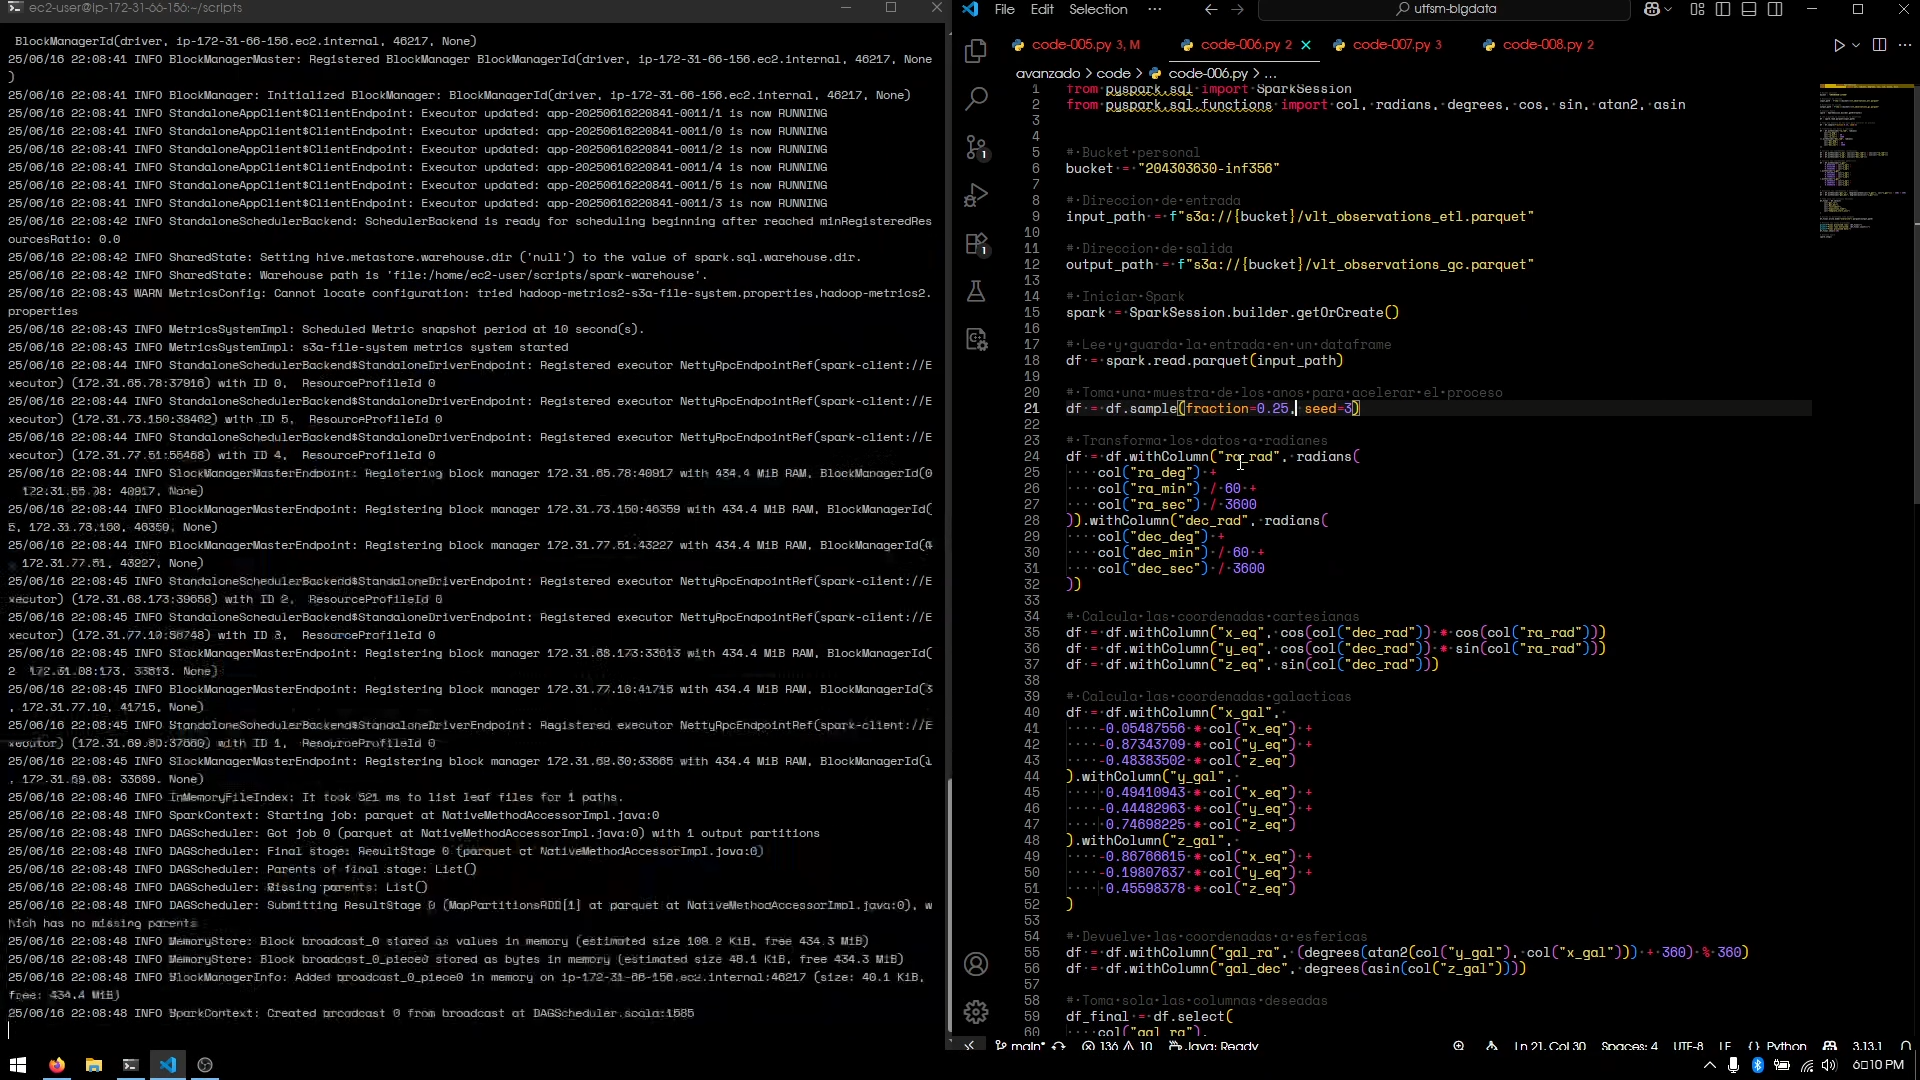
\includegraphics[height=5cm]{32-figura-1.PNG}
    \caption{Spark procesando los datos mientras explico el codigo}
\end{figure}

\begin{figure}[H]
    \centering
    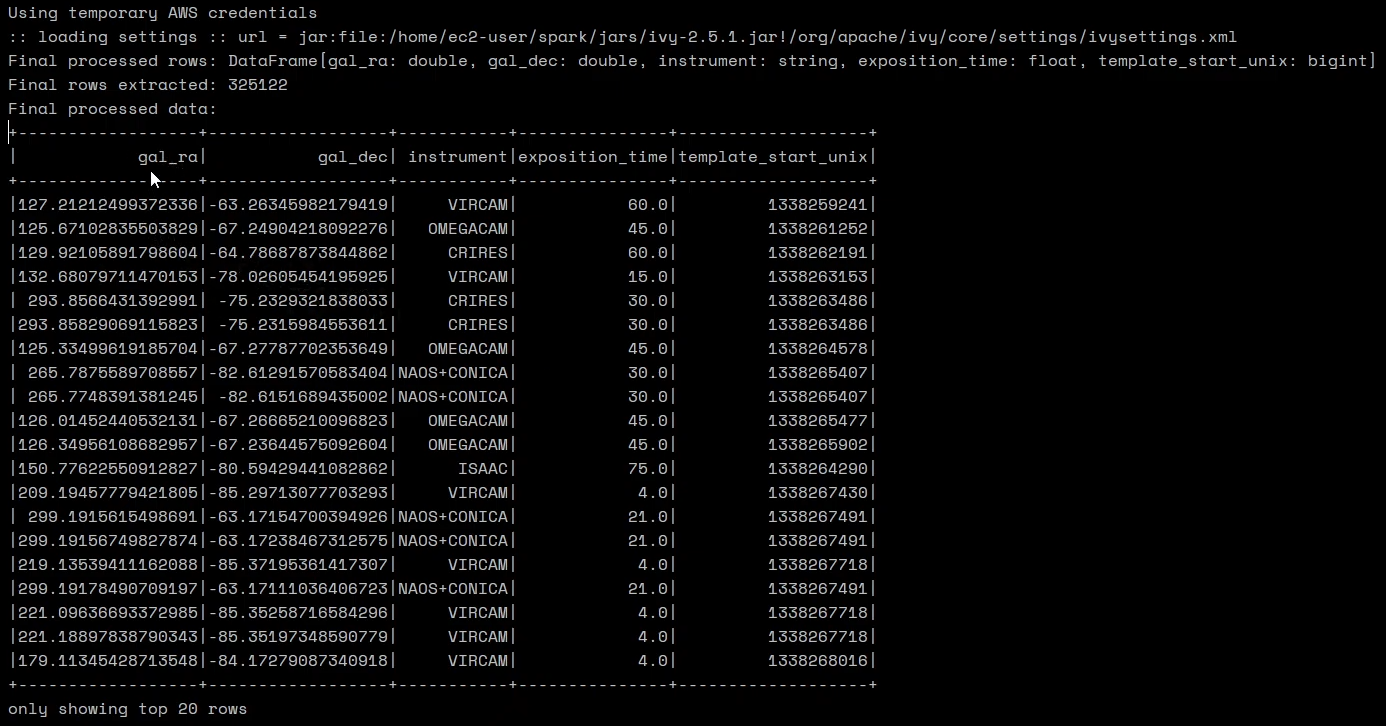
\includegraphics[height=5cm]{32-figura-final.PNG}
    \caption{Dataframe resultante tras procesar los datos}
\end{figure}

\newpage
\begin{code}[H]
    \lstinputlisting[style=pythonstyle, caption={Código utilizado para el cálculo de coordenadas galácticas}, label={lst:006}]{code/code-006-cut-1.py}
\end{code}
\newpage
\begin{code}[H]
    \lstinputlisting[style=pythonstyle, caption={Código utilizado para el cálculo de coordenadas galácticas}, label={lst:006}]{code/code-006-cut-2.py}
\end{code}
\newpage

\subsection{Segmentación temporal}

A partir del archivo con coordenadas galácticas, se segmentaron los datos por año y por semana del año, considerando como primera semana la que contiene el primer lunes. Las fechas anteriores a ese lunes fueron asociadas al año anterior.

Se transformó la fecha desde formato Unix a calendario, se identificaron los años distintos y el primer lunes correspondiente para cada uno. Luego, se asignaron las observaciones a su semana correspondiente y se ajustó el año cuando era necesario.

Finalmente, los datos fueron almacenados en formato \texttt{Parquet} dentro del directorio \texttt{partition/}, organizados por carpeta de año. Cada año contiene un archivo con todos sus datos (\texttt{vlt\_observations\_XXXX.parquet}) y una subcarpeta \texttt{weeks/} con archivos semanales por año.

Es importante recalcar que justamente al ejecutar este codigo, AWS se colapso y me echo del cluster de Spark, e inclusi en el video se muestra como no se alcanzo a procesar toda la data.

Ya que este procedimiento era bastante largo, decidir revisar el bucket para ver si proceso algo de los datos entregados, los nodos alcanzaron a agrupar solo las semanas del 2018, sin embargo se podia
ver que se cumplia el formato pedido de las fechas y numeracion de semanas, por lo que decidi dejarlo hasta ahi y seguir con el punto siguiente.

\begin{itemize}
  \item Ejecucion y mi explicacion del codigo: {\color{blue}\href{https://youtu.be/GdrpnyFULTI?si=vEHhc2fKoWvcQzTY&t=547}{enlace}}.
  \item Momento en donde AWS me echa del entorno: {\color{blue}\href{https://youtu.be/GdrpnyFULTI?si=wfYQl2w1CQLTAboK&t=686}{enlace}}.
  \item Evidencia de que los datos se guardaron: {\color{blue}\href{https://youtu.be/GdrpnyFULTI?si=1imVLcvU_TyfZjSQ&t=940}{enlace}}.
\end{itemize}

\begin{figure}[H]
    \centering
    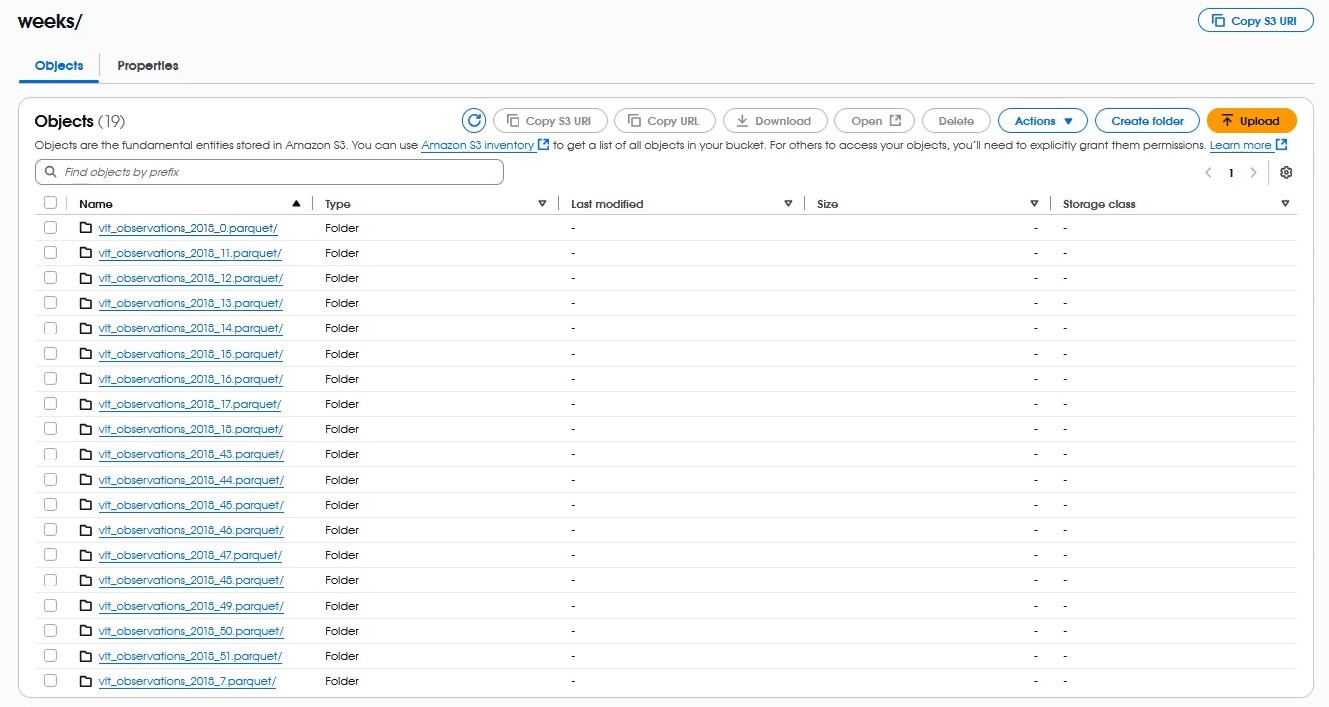
\includegraphics[height=5cm]{33-figura-final.PNG}
    \caption{Pantallazo del Bucket S3 resultante tras procesar los datos}
\end{figure}

\newpage

\begin{code}[H]
    \lstinputlisting[style=pythonstyle, caption={Código utilizado para segmentación temporal de datos}, label={lst:007}]{code/code-007-cut-1.py}
\end{code}

\newpage

\begin{code}[H]
    \lstinputlisting[style=pythonstyle, caption={Código utilizado para segmentación temporal de datos}, label={lst:007}]{code/code-007-cut-2.py}
\end{code}

\subsection{Conteo de observaciones}

El último paso fue generar un conteo de observaciones agrupadas por instrumento y por bloques de 10 grados del cielo tanto horizontal como verticalmente. A partir del archivo con coordenadas galácticas, se agruparon los datos según el centro de cada celda angular de 10x10 grados.

En cada celda, se sumó el tiempo total de exposición en lugar de mantener los valores individuales, y se descartó el campo \texttt{template\_start}. El archivo de salida se guardó con el mismo nombre que el archivo de entrada, pero agregando \texttt{.count} antes de la extensión.

Evidencia del desarrollo a modo de images y enlace a la seccion del video con la demostracion ({\color{blue}\href{https://youtu.be/GdrpnyFULTI?si=if9d7dEC7Wyjnwij&t=1303}{enlace}}).

\begin{figure}[H]
    \centering
    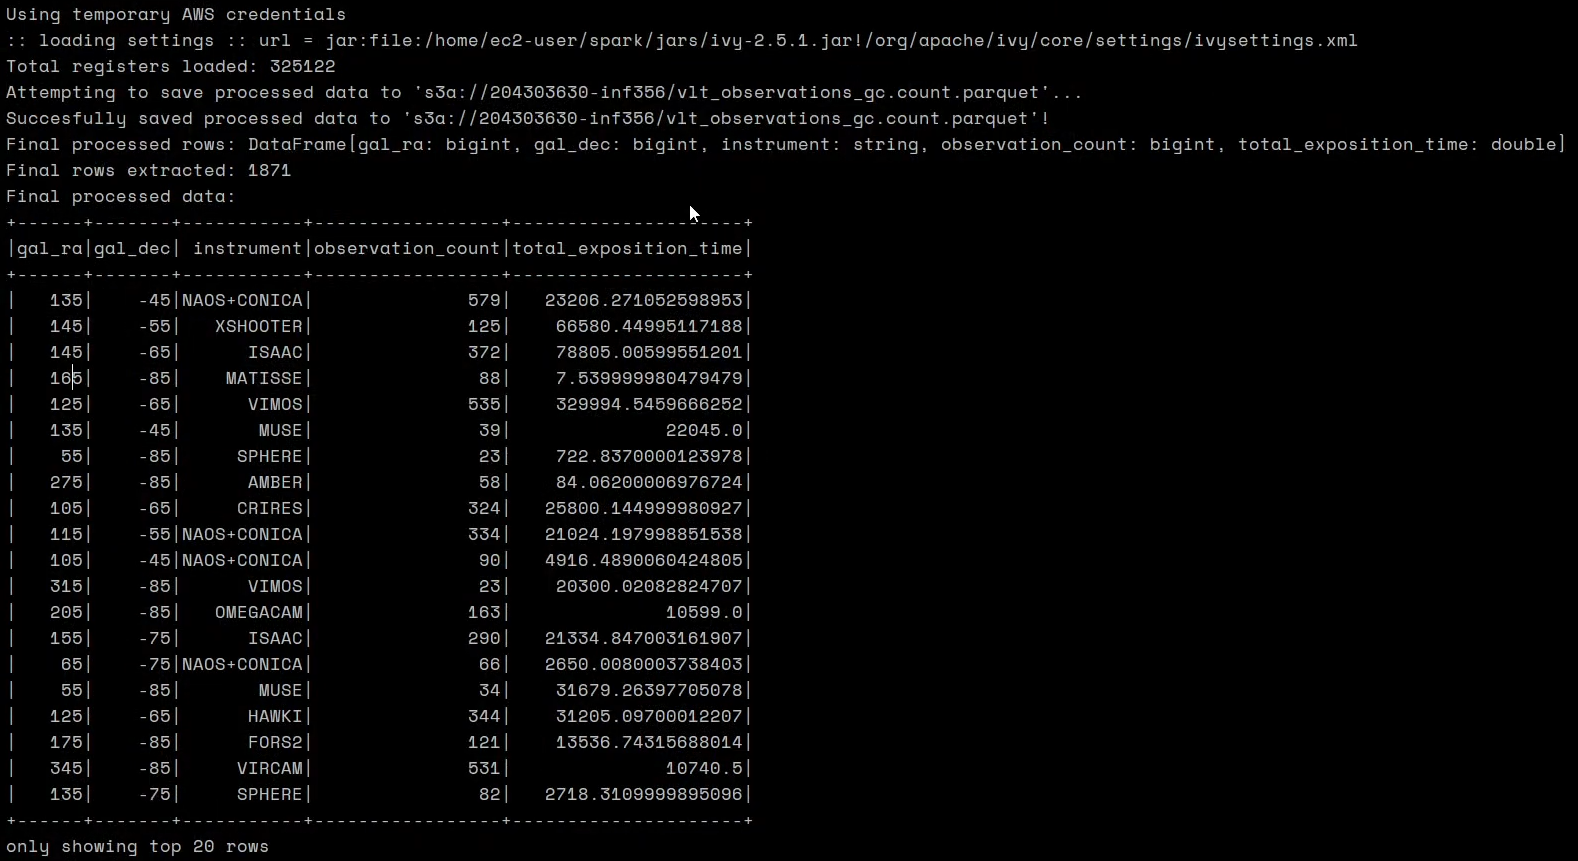
\includegraphics[height=5cm]{34-figura-final.PNG}
    \caption{Dataframe resultante tras procesar los datos}
\end{figure}

\newpage

\begin{code}[H]
    \lstinputlisting[style=pythonstyle, caption={Código utilizado para segmentación temporal de datos}, label={lst:007}]{code/code-008.py}
\end{code}
\newpage

\end{document}
